\documentclass{beamer}

\usepackage{../cppenv}
\usepackage{../recdefs}

\usetheme{Singapore}

\title{CS100 Recitation 9}
\author{GKxx}
\date{April 18, 2022}

\AtBeginSubsection{
    \begin{frame}{Contents}
        \tableofcontents[currentsection, currentsubsection]
    \end{frame}
}

\begin{document}

\begin{frame}
    \maketitle
\end{frame}

\begin{frame}{Contents}
    \tableofcontents
\end{frame}

\section{Inheritance and Polymorphism}

\subsection{Inheritance}

\begin{frame}{Defining a Subclass}
    An item for sale:
    \begin{itemize}
        \item \ttt{std::string name;}
        \item \ttt{double price;}
        \item \ttt{std::string get\_name() const;}
        \item \ttt{double net\_price(std::size\_t n) const;}
    \end{itemize}
    A discounted item \textbf{is an} item, and has some more information:
    \begin{itemize}
        \item \ttt{std::size\_t min\_quantity;}
        \item \ttt{double discount;}
    \end{itemize}
    The net price for such item is \ttt{n * price} if \ttt{n < min\_quantity}, or \ttt{n * discount * price} otherwise.
\end{frame}

\begin{frame}{Defining a Subclass}
    Things to consider:
    \begin{itemize}
        \item Does your class need a default constructor?
        \begin{itemize}
            \item If so, what should be a reasonable behavior?
            \item What will happen if not?
        \end{itemize}
        \item Does your class need special copy-control?
        \begin{itemize}
            \item Seems not.
            \item But what if we have another thing called a \ttt{Basket}...?
            \item What if every item has a unique id...?
        \end{itemize}
        \item What value should \ttt{discount} have to represent `20\% off'?
    \end{itemize}
\end{frame}

\begin{frame}{\bluett{protected} members}
    A \bluett{protected} member is private, except that it is accessible in subclasses.
    \begin{itemize}
        \item \ttt{price} is accessible in \ttt{Discounted\_item}.
        \item Should \ttt{name} be \bluett{protected} or \bluett{private}?
        \begin{itemize}
            \item \private is ok if the subclass doesn't (shouldn't) modify it. It is accessible through the public \ttt{get\_name} interface.
            \item \bluett{protected} is also reasonable.
        \end{itemize}
    \end{itemize}
    The core idea is to \textbf{separate implementation details and interfaces}.
\end{frame}

\begin{frame}[fragile]{Inheritance}
    By defining \ttt{Discounted\_item} to be a subclass of \ttt{Item}, \textbf{every object of \ttt{Discounted\_item} contains an object of \ttt{Item}}.
    \begin{itemize}
        \item Every data member and member function, except the constructors, are inherited, no matter what access level they have.
        \item What can we derive from this?
        \begin{itemize}
            \item When constructing an object of a subclass, one of the ctors of the base class must be called before initializing the members that the subclass declares.
            \item The dtor of the subclass must call the dtor of the base class (automatically) after the members of the subclass are destroyed.
            \item \ttt{\blue{sizeof}(Derived) >= \blue{sizeof}(Base)}.
        \end{itemize}
    \end{itemize}
\end{frame}

\begin{frame}{Inheritance}
    Core ideas of inheritance:
    \begin{itemize}
        \item Every sub-object contains an object of the base class.
        \item The father has his own ways of doing things, which children cannot affect!
    \end{itemize}
\end{frame}

\begin{frame}[fragile]{Inheritance and Constructors}
    \begin{cpp}
class Discounted_item : public Item {
  std::size_t min_quantity = 0;
  double discount = 1.0;
 public:
  Discounted_item(const std::string &s, double p,
                  std::size_t qty, double disc)
      : Item(s, p), min_quantity(qty), discount(disc) {}
  // other members
};
    \end{cpp}
    \begin{itemize}
        \item What if we don't call the ctor of the base class explicitly?
        \item Can we directly initialize the members of the base class?
        \begin{cpp}
Discounted_item(const std::string &s, double p,
                std::size_t qty, double disc)
    : name(s), price(p), min_quantity(qty),
      discount(disc) {}
        \end{cpp}
    \end{itemize}
\end{frame}

\begin{frame}[fragile]{Inheritance and Constructors}
    \begin{columns}
        \begin{column}{0.6\linewidth}
            Ctors are not automatically inherited, but we can inherit them explicitly:
            \begin{cpp}
class Binary_node {
 protected:
  Expr_node *lhs, *rhs;
  Binary_node(Expr_node *left,
      Expr_node *right)
      : lhs(left), rhs(right) {}
  // other members
};
class Plus_node
    : public Binary_node {
  using Binary_node::Binary_node;
  // other members
};
            \end{cpp}
        \end{column}
        \begin{column}{0.5\linewidth}
            then \ttt{Plus\_node} has a constructor
            \begin{cpp}
Plus_node(Expr_node *left, Expr_node *right)
  : Binary_node(left, right) {}
            \end{cpp}
            and we can call it by
            \begin{cpp}
Plus_node pn(a, b);
auto pnp
    = new Plus_node(a, b);
            \end{cpp}
        \end{column}
    \end{columns}
\end{frame}

\begin{frame}{Inheritance and Constructors}
    \begin{itemize}
        \item Default ctor and copy ctor won't be inherited by a \bluett{using} declaration. \red{(Why?)}
        \item All the ctors (except default ctor and copy ctor) are inherited by a \bluett{using} declaration. But the subclass can rewrite some.
        \begin{itemize}
            \item If the subclass has a ctor which has the same parameters as one of the ctors of the base class, then this ctor is hiding the corresponding one of the base class.
        \end{itemize}
        \item The access-level will be preserved. \red{(Why?)}
        \item The \bluett{explicit} attribute, if any, is also preserved.
        \item How will the inherited ctors initialize the members of the subclass?
    \end{itemize}
\end{frame}

\begin{frame}{Inheritance and \bluett{friend}s}
    Friendship cannot be inherited.
    \begin{itemize}
        \item Are you getting along well with your father's friends?
    \end{itemize}
\end{frame}

\begin{frame}{Inheritance and Copy-control}
    We will talk about this later...
\end{frame}

\subsection{Dynamic Binding}

\begin{frame}[fragile]{Upcasting}
    A reference or pointer to base class can be bound to an object of subclass. \red{(Why?)}
    \begin{cpp}
Discounted_item di = some_value();
Item &ir = di;  // Treat di as an Item object
Item *ip = &di;
    \end{cpp}
    But on such references or pointers, only the members of base class are accessible. \red{(Why?)}
\end{frame}

\begin{frame}[fragile]{Upcasting: Example}
    \begin{cpp}
inline void print_info(const Item &item) {
  std::cout << "Name: " << item.get_name()
            << ", price: " << item.net_price(1)
            << std::endl;
}
// in main
Discounted_item di = some_value();
Item i = some_other_value();
print_info(di);
print_info(i);
    \end{cpp}
\end{frame}

\begin{frame}[fragile]{Static Type and Dynamic Type}
    \begin{itemize}
        \item \textbf{static type} of an expression: The type known at compile-time.
        \item \textbf{dynamic type} of an expression: The real type of the object that the expression or variable is representing. \textbf{Known at runtime}.
    \end{itemize}
    \begin{cpp}
Discounted_item di = some_value();
Item &ir = di; // ir has static type Item &,
               // but dynamic type Discounted_item.
    \end{cpp}
\end{frame}

\begin{frame}[fragile]{Static Type and Dynamic Type}
    \begin{cpp}
inline void print_info(const Item &item) {
  std::cout << "Name: " << item.get_name()
            << ", price: " << item.net_price(1)
            << std::endl;
}
    \end{cpp}
    The static type of \ttt{item} is \const\ttt{Item \&}, but the dynamic type is unknown.
\end{frame}

\begin{frame}[fragile]{\virtual Functions}
    \begin{cpp}
inline void print_info(const Item &item) {
  std::cout << "Name: " << item.get_name()
            << ", price: " << item.net_price(1)
            << std::endl;
}
    \end{cpp}
    Which \ttt{net\_price} is called?
\end{frame}

\begin{frame}[fragile]{\virtual Functions}
    \begin{cpp}
class Item {
 public:
  virtual double net_price(std::size_t n) const;
  // other members
};
class Discounted_item : public Item {
 public:
  virtual double net_price(std::size_t n) const override;
  // other members
};
    \end{cpp}
\end{frame}

\begin{frame}{\virtual Functions}
    \begin{itemize}
        \item The dynamic type of parameter \ttt{item} is runtime-determined.
        \item Since \ttt{net\_price} is a \virtual function, which one is called is determined at \textbf{runtime}, so that the correct version is called.
        \item \textbf{late-binding}, or \textbf{dynamic-binding}.
    \end{itemize}
\end{frame}

\begin{frame}{Overriding a \virtual Function}
    To \override a \virtual function,
    \begin{itemize}
        \item The function must have parameters the same as the function in the base class has.
        \item The return-type of the function should be either \textbf{identical to} or \textbf{covariant with} \red{(What's this?)} that of the corresponding function in the base class.
        \item Don't forget the \const qualifier!
    \end{itemize}
    To make sure that your function overrides the one in the base class, use the \override keyword.
\end{frame}

\begin{frame}{Overriding a \virtual Function}
    \begin{itemize}
        \item An overriding function is still \bluett{virtual}, even if not explicitly declared.
        \item The best practice is to explicitly write `\bluett{virtual}' and `\bluett{override}'.
        \begin{itemize}
            \item The \override keyword lets the compiler check and report if the function is not actually overriding.
        \end{itemize}
        \item Distinguish between \textbf{overriding}, \textbf{overloading} and `\textbf{hiding}'.
        \begin{itemize}
            \item Avoid confusing cases in your program! Don't invite troubles for yourself.
        \end{itemize}
    \end{itemize}
\end{frame}

\begin{frame}[fragile]{\virtual Destructors}
    \begin{cpp}
Base *bp = some_value();
delete bp;
    \end{cpp}
    which destructor should be called by `\bluett{delete }\ttt{bp}'?
    \pause
    \begin{itemize}
        \item To make dynamic binding work correctly, the destructors must be \bluett{virtual}!
        \item The synthesized destructor is \textbf{non-virtual}, but we can:
        \begin{cpp}
virtual ~Base() = default;
        \end{cpp}
        \item If the dtor of the base class is \bluett{virtual}, the synthesized destructor is also \bluett{virtual}.
    \end{itemize}
\end{frame}

\begin{frame}[fragile]{Inheritance and Copy-control}
    Remember to copy the base part correctly! One possible way:
    \begin{cpp}
class Derived : public Base {
 public:
  Derived(const Derived &d)
    : Base(d), /* members of Derived */ {}
  Derived &operator=(const Derived &d) {
    Base::operator=(d);
    // copy members of Derived
    return *this;
  }
};
    \end{cpp}
\end{frame}

\begin{frame}{Synthesized Copy-control Functions}
    \begin{itemize}
        \item When will the compiler synthesize a copy-control function?
        \item What's the behavior of them?
        \item When will the compiler mark them as \blue{deleted}?
        \item What about default ctors?
    \end{itemize}
\end{frame}

\begin{frame}[fragile]{Slicing}
    Suppose \ttt{Base} and \ttt{Derived} have a \virtual function \ttt{foo}.
    \begin{cpp}
Derived d = some_value();
Base b = d;
b.foo();    // Base::foo or Derived::foo?
    \end{cpp}
    When using an object of a subclass to initialize or assign to an object of the base class, the copy-ctor or copy-assignment operator \textbf{of the base class} is called.
    \begin{itemize}
        \item Therefore, the sub-part of the object is ignored, or \textbf{sliced down}.
        \item Dynamic binding won't happen.
    \end{itemize}
\end{frame}

\begin{frame}[fragile]{Downcasting}
    \begin{cpp}
Base *bp = new Derived{};
    \end{cpp}
    We cannot access the members of the subclass through a pointer to the base class. We need a \textbf{downcasting}.
    \begin{itemize}
        \item As long as the following conditions are satisfied, you can make a downcasting:
        \begin{itemize}
            \item The pointer or reference to the base class is \textbf{indeed} bound to an object of the subclass.
            \item The base class and the subclass are polymorphic, which means that there is at least one \virtual function.
        \end{itemize}
        \item You can make a downcasting by \bluett{dynamic\_cast}:
        \begin{cpp}
Derived *dp = dynamic_cast<Derived *>(bp);
Derived &dr = dynamic_cast<Derived &>(*bp);
        \end{cpp}
    \end{itemize}
\end{frame}

\begin{frame}{Downcasting}
    \begin{itemize}
        \item \bluett{dynamic\_cast} may have a significant runtime cost.
        \item Several common ways to avoid \bluett{dynamic\_cast}, like writing a group of \virtual functions.
        \item \textit{Effective C++} Item 27 talks about type-casting.
        \item \textit{More Effective C++} Item 31 talks about some more complicated cases: Making functions virtual with respect to more than one object.
    \end{itemize}
    \begin{notice}
        Avoid \bluett{dynamic\_cast}, especially in performance-sensitive code.
    \end{notice}
\end{frame}

\subsection{Abstract Base Classes}

\begin{frame}[fragile]{Pure \virtual Functions}
    By defining a function to be \ttt{=0}, it is defined as a \textbf{pure virtual} function.
    \begin{itemize}
        \item A class with at least one pure virtual function is an \textbf{abstract class}.
        \item A pure virtual function can be overridden in a subclass. But if it is not overridden, the subclass is still abstract.
        \item Creating objects of a type that is an abstract class is \textbf{not allowed}.
    \end{itemize}
    \blue{Generally, virtual functions in the base class that do not have a reasonable behavior should be pure virtual, and such class should be abstract.}
\end{frame}

\begin{frame}{Example: Greedy Snake}
    \begin{columns}
        \begin{column}{0.5\linewidth}
            ``A super-speed game is a game.''
            \begin{figure}[h]
                \centering
                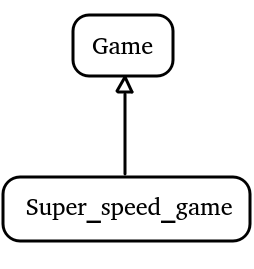
\includegraphics[scale=0.5]{figures/snake_original.png}
            \end{figure}
        \end{column}
        \begin{column}{0.5\linewidth}
            ``A classic-mode game is a game. A super-speed game is also a game.''
            \begin{figure}[h]
                \centering
                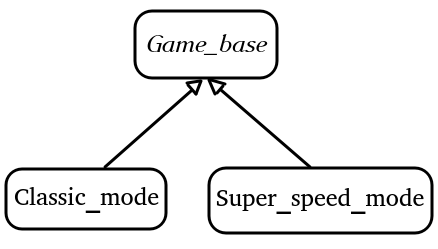
\includegraphics[width=\textwidth]{figures/snake_new.png}
            \end{figure}
        \end{column}
    \end{columns}
    It turns out that the super-speed mode has too many differences from the classic-mode, so I \textbf{refactored} the program according to the diagram on the right.
\end{frame}

\begin{frame}{Which One is Better?}
    \begin{columns}
        \begin{column}{0.5\linewidth}
            \begin{figure}[h]
                \centering
                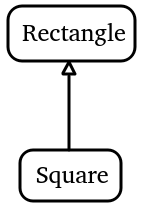
\includegraphics[scale=0.6]{figures/shape_original.png}
            \end{figure}
        \end{column}
        \begin{column}{0.5\linewidth}
            \begin{figure}[h]
                \centering
                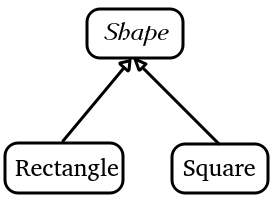
\includegraphics[scale=0.6]{figures/shape_new.png}
            \end{figure}
        \end{column}
    \end{columns}
\end{frame}

\begin{frame}{Which One is Better?}
    \begin{itemize}
        \item ``A square \textbf{is a} rectangle'' is correct, but sometimes this is deceptive. (\textit{Effective C++} Item 32, very important)
        \item The structure on the right can be extended easily: (\textbf{reusability})
        \begin{figure}[h]
            \centering
            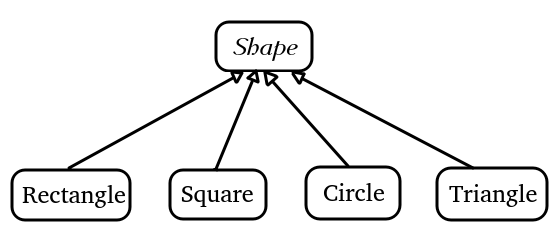
\includegraphics[scale=0.6]{figures/shape_extended.png}
        \end{figure}
    \end{itemize}
\end{frame}

\begin{frame}[fragile]{A Pure \virtual Destructor}
    Sometimes a class should be abstract, but there seems to be no reasonable choice over which function should be pure virtual.
    \pause
    \begin{itemize}
        \item Define the destructor to be pure virtual, and provide another definition.
    \end{itemize}
    \begin{cpp}
class Base {
 public:
  virtual ~Base() = 0;
};
Base::~Base() {}
    \end{cpp}
    In fact, we can provide definitions for pure virtual functions.
\end{frame}

\begin{frame}[fragile]{More on Inheritance...}
    \begin{itemize}
        \item There is still one thing that is magic to us: the `\bluett{public}' keyword:
        \begin{cpp}
class Discounted_item : public Item {};
        \end{cpp}
        \item \public inheritance models `is-a', while \private inheritance models `is-implemented-in-terms-of'. What's that?
    \end{itemize}
\end{frame}

\section{More on Functions}

\subsection{Default Arguments}

\begin{frame}[fragile]{Default Arguments}
    \begin{cpp}
void create_window(std::size_t height = 24,
                   std::size_t width = 80) {
  // create a window with given height and width
}
    \end{cpp}
    If the caller omit the `\ttt{width}' argument
    \begin{cpp}
create_window(30);
    \end{cpp}
    then \ttt{width} will be set to default value \ttt{80}.
    If both arguments are omitted
    \begin{cpp}
create_window();
    \end{cpp}
    then \ttt{height} is set to \ttt{24} and \ttt{width} \ttt{80}.
\end{frame}

\begin{frame}[fragile]{Default Arguments}
    \begin{itemize}
        \item Only the last few parameters can have default arguments.
        \begin{cpp}
void fun(int a = 42, int b); // Error
        \end{cpp}
        \item Functions that have default arguments will be treated as \textbf{overloading functions}. For the \ttt{create\_window} function, it is the same as
        \begin{cpp}
void create_window();
void create_window(std::size_t height);
void create_window(std::size_t height,
                   std::size_t width);
        \end{cpp}
    \end{itemize}
\end{frame}

\begin{frame}[fragile]{Default Arguments}
    Member functions can also have default arguments:
    \begin{cpp}
class Vector {
 public:
  Vector(std::size_t n, int val = 0)
      : m_size(n), m_capacity(n),
        m_data(new int[n]{}) {
    for (std::size_t i = 0; i < n; ++i)
      m_data[i] = val;
  }
  // other members
};
    \end{cpp}
    It will be treated as if there are two constructors
    \begin{cpp}
Vector::Vector(std::size_t);
Vector::Vector(std::size_t, int);
    \end{cpp}
\end{frame}

\begin{frame}[fragile]{Default Argument Declaration}
    A function may be declared multiple times, but default arguments should \textbf{not} be redeclared.
    \begin{cpp}
class Vector {
 public:
  Vector(std::size_t n, int val = 0);
};
Vector::Vector(std::size_t n, int val = 0) // Error.
    : m_size(n), m_capacity(n), m_data(new int[n]{}) {
  std::fill_n(m_data, n, val);
}
    \end{cpp}
\end{frame}

\begin{frame}[fragile]{Default Argument Declaration}
    A function may be declared multiple times, but default arguments should \textbf{not} be redeclared. \red{(Why?)}
    \begin{cpp}
class Vector {
 public:
  Vector(std::size_t n, int val = 0);
};
Vector::Vector(std::size_t n, int val) // Correct.
    : m_size(n), m_capacity(n), m_data(new int[n]{}) {
  std::fill_n(m_data, n, val);
}
    \end{cpp}
\end{frame}

\begin{frame}[fragile]{Default Argument Declaration}
    Although it seems weird, subsequent declarations can have additional default arguments.
    \begin{cpp}
void create_window(std::size_t height,
                   std::size_t width = 80);
void craete_window(std::size_t height = 24, // OK.
                   std::szie_t width) {
  // ...
}
    \end{cpp}
    Defaults can be specified only when all parameters to the right already have defaults.
\end{frame}

\subsection{Passing Command-Line Arguments}

\begin{frame}[fragile]{Command-Line Arguments}
    \textbf{Suppose you are the author of \ttt{g++}}. When the user type\\
    \ttt{g++ -o hello hello.cpp}\\
    in the terminal, there should be a way to let your program get this command.
    \pause
    \begin{cpp}
int main(int argc, char **argv) {
  // ...
}
    \end{cpp}
    \begin{itemize}
        \item \ttt{argv} is an array of strings. In this example, \ttt{argv = \{"g++", "-o", "hello", "hello.cpp"\}}.
        \item \ttt{argc} is the number of strings in the array \ttt{argv}.
        \item \ttt{char *argv[]} is the same as \ttt{char **argv}.
    \end{itemize}
\end{frame}

\begin{frame}[fragile]{Command-Line Arguments}
    \textbf{The only two} correct versions of the \ttt{main} function:
    \begin{cpp}
int main();
int main(int argc, char **argv);
    \end{cpp}
\end{frame}

\section{Aids for Debugging}

\begin{frame}[fragile]{Assertion}
    \begin{cpp}
#include <cassert>
int main() {
  int a, b;
  std::cin >> a >> b;
  assert(b != 0);
  int c = a / b;
  // ...
}
    \end{cpp}
    C++11 also provides compile-time assertion \bluett{static\_assert}, but it's too early for you now... (We used this in Problem 2 to detect whether your \ttt{Shape} class is abstract.)
\end{frame}

\begin{frame}[fragile]{Some Helpful Macros}
    To disable assertions, we can use the \ttt{NDEBUG} macro.
    \begin{cpp}
int main() {
  int a, b;
  std::cin >> a >> b;
#define NDEBUG
  assert(b != 0); // This assertion will not be performed.
#undef NDEBUG
  assert(b != 0); // This assertion will be performed.
  // ...
}
    \end{cpp}
\end{frame}

\begin{frame}[fragile]{Some Helpful Macros}
    \begin{itemize}
        \item \ttt{\_\_LINE\_\_}: \bluett{int}, the line number.
        \item \ttt{\_\_func\_\_}: \const\bluett{char }\ttt{[]}, the name of the current function.
        \item \ttt{\_\_FILE\_\_}: \const\bluett{char }\ttt{[]}, the name of the current file.
        \item \ttt{\_\_TIME\_\_}: \const\bluett{char }\ttt{[]}, the current time.
    \end{itemize}
\end{frame}

\section{Type Aliases}

\begin{frame}[fragile]{New-style Alias Declaration}
    \begin{cpp}
using LL = long long;
    \end{cpp}
    The new-style type alias declaration is more clear:
    \begin{cpp}
typedef int arr_t[10];
using arr_t = int[10];
    \end{cpp}
    The \bluett{using} type alias declaration can also be a template, but \bluett{typedef} cannot.
\end{frame}

\begin{frame}[fragile]{Type Alias Member}
    \begin{columns}
        \begin{column}{0.6\linewidth}
            \begin{cpp}
class Vector {
 public:
  using size_type = std::size_t;
  using value_type = int;
  using pointer = int *;
  using reference = int &;
  // other members
};
int main() {
  Vector v = some_value();
  for (Vector::size_type i = 0;
       i < v.size(); ++i)
    // do something
}
            \end{cpp}
        \end{column}
        \begin{column}{0.5\linewidth}
            \begin{itemize}
                \item Access modifiers also apply to type alias members.
                \item To access a type alias member, use \textit{class-name}\ttt{::}\textit{type-member}.
            \end{itemize}
        \end{column}
    \end{columns}
\end{frame}

\end{document}